\documentclass[tikz,border=8pt]{standalone}
% Shared look for every TikZ diagram. Load with % Shared look for every TikZ diagram. Load with % Shared look for every TikZ diagram. Load with \input{../../tools/tikz-style.tex}
\usepackage[T1]{fontenc}
\usepackage{lmodern}
\renewcommand{\sfdefault}{lmr}  % diagrams use the same serif as the text
\usetikzlibrary{arrows.meta, positioning, shapes.geometric, calc, fit, backgrounds}
\definecolor{cblue}{HTML}{4C78A8}
\definecolor{corange}{HTML}{F58518}
\definecolor{cgreen}{HTML}{54A24B}
\definecolor{cred}{HTML}{E45756}
\definecolor{cpurple}{HTML}{B279A2}
\definecolor{cgrey}{HTML}{6B6B6B}
\tikzset{
  every picture/.style={font=\sffamily, line width=1.2pt},
  box/.style={draw=#1, fill=#1!12, rounded corners=4pt, align=center, inner sep=7pt, minimum height=1.1cm},
  box/.default=cgrey,
  arrow/.style={-{Stealth[length=3mm]}, draw=cgrey, line width=1.4pt},
  title/.style={font=\sffamily\bfseries\Large},
  note/.style={font=\sffamily\small, text=cgrey, align=center},
}
\AtBeginDocument{\hyphenpenalty=10000 \exhyphenpenalty=10000}

\usepackage[T1]{fontenc}
\usepackage{lmodern}
\renewcommand{\sfdefault}{lmr}  % diagrams use the same serif as the text
\usetikzlibrary{arrows.meta, positioning, shapes.geometric, calc, fit, backgrounds}
\definecolor{cblue}{HTML}{4C78A8}
\definecolor{corange}{HTML}{F58518}
\definecolor{cgreen}{HTML}{54A24B}
\definecolor{cred}{HTML}{E45756}
\definecolor{cpurple}{HTML}{B279A2}
\definecolor{cgrey}{HTML}{6B6B6B}
\tikzset{
  every picture/.style={font=\sffamily, line width=1.2pt},
  box/.style={draw=#1, fill=#1!12, rounded corners=4pt, align=center, inner sep=7pt, minimum height=1.1cm},
  box/.default=cgrey,
  arrow/.style={-{Stealth[length=3mm]}, draw=cgrey, line width=1.4pt},
  title/.style={font=\sffamily\bfseries\Large},
  note/.style={font=\sffamily\small, text=cgrey, align=center},
}
\AtBeginDocument{\hyphenpenalty=10000 \exhyphenpenalty=10000}

\usepackage[T1]{fontenc}
\usepackage{lmodern}
\renewcommand{\sfdefault}{lmr}  % diagrams use the same serif as the text
\usetikzlibrary{arrows.meta, positioning, shapes.geometric, calc, fit, backgrounds}
\definecolor{cblue}{HTML}{4C78A8}
\definecolor{corange}{HTML}{F58518}
\definecolor{cgreen}{HTML}{54A24B}
\definecolor{cred}{HTML}{E45756}
\definecolor{cpurple}{HTML}{B279A2}
\definecolor{cgrey}{HTML}{6B6B6B}
\tikzset{
  every picture/.style={font=\sffamily, line width=1.2pt},
  box/.style={draw=#1, fill=#1!12, rounded corners=4pt, align=center, inner sep=7pt, minimum height=1.1cm},
  box/.default=cgrey,
  arrow/.style={-{Stealth[length=3mm]}, draw=cgrey, line width=1.4pt},
  title/.style={font=\sffamily\bfseries\Large},
  note/.style={font=\sffamily\small, text=cgrey, align=center},
}
\AtBeginDocument{\hyphenpenalty=10000 \exhyphenpenalty=10000}

% Section 2 worked examples. Top: disc of radius 1 with x = (1,0), y = (0,1); midpoint (0.5, 0.5) has length 0.71 <= 1,
% inside. Ring 1 <= length <= 2 with x = (1.5,0), y = (-1.5,0); midpoint (0,0) has length 0 < 1, outside.
% Bottom: the overlap of two convex discs is convex; their union is not (the segment crosses empty space).
\begin{document}
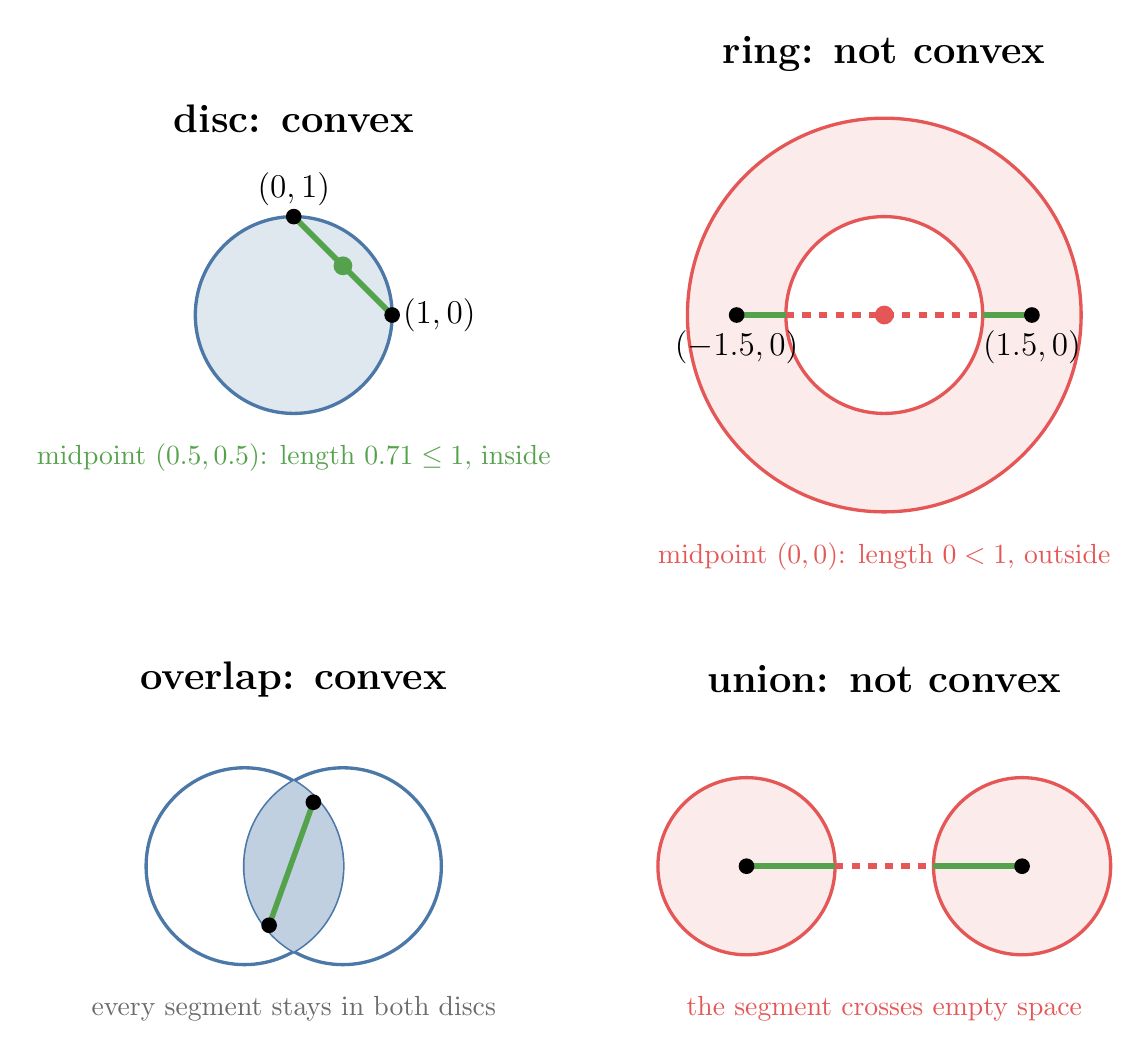
\begin{tikzpicture}[scale=1.25, every node/.append style={font=\large}, dot/.style={circle, fill=black, inner sep=2pt}]
  % ---- disc
  \node[title] at (0,2.0) {disc: convex};
  \fill[cblue!18, draw=cblue] (0,0) circle (1);
  \draw[cgreen, line width=2pt] (1,0) node[dot]{} -- (0,1) node[dot]{};
  \node[right] at (1,0) {$(1, 0)$}; \node[above] at (0,1) {$(0, 1)$};
  \node[circle, fill=cgreen, inner sep=2.4pt] (m) at (0.5,0.5) {};
  \node[note, text=cgreen, font=\normalsize] at (0.0,-1.45) {midpoint $(0.5, 0.5)$: length $0.71 \le 1$, inside};
  % ---- ring
  \begin{scope}[xshift=6cm]
    \node[title] at (0,2.65) {ring: not convex};
    \fill[cred!12, draw=cred, even odd rule] (0,0) circle (2) (0,0) circle (1);
    \draw[cgreen, line width=2pt] (-1.5,0) node[dot]{} -- (-1,0);
    \draw[cred, line width=2pt, dashed] (-1,0) -- (1,0);
    \draw[cgreen, line width=2pt] (1,0) -- (1.5,0) node[dot]{};
    \node[below] at (1.5,-0.05) {$(1.5, 0)$}; \node[below] at (-1.5,-0.05) {$(-1.5, 0)$};
    \node[circle, fill=cred, inner sep=2.4pt] at (0,0) {};
    \node[note, text=cred, font=\normalsize] at (0,-2.45) {midpoint $(0, 0)$: length $0 < 1$, outside};
  \end{scope}
  % ---- overlap and union
  \begin{scope}[yshift=-5.6cm]
    \node[title] at (0,1.9) {overlap: convex};
    \draw[cblue] (-0.5,0) circle (1); \draw[cblue] (0.5,0) circle (1);
    \begin{scope} \clip (-0.5,0) circle (1); \fill[cblue!35] (0.5,0) circle (1); \end{scope}
    \draw[cgreen, line width=2pt] (-0.25,-0.6) node[dot]{} -- (0.2,0.65) node[dot]{};
    \node[note, font=\normalsize] at (0,-1.45) {every segment stays in both discs};
  \end{scope}
  \begin{scope}[xshift=6cm, yshift=-5.6cm]
    \node[title] at (0,1.9) {union: not convex};
    \fill[cred!12, draw=cred] (-1.4,0) circle (0.9); \fill[cred!12, draw=cred] (1.4,0) circle (0.9);
    \draw[cgreen, line width=2pt] (-1.4,0) node[dot]{} -- (-0.5,0);
    \draw[cred, line width=2pt, dashed] (-0.5,0) -- (0.5,0);
    \draw[cgreen, line width=2pt] (0.5,0) -- (1.4,0) node[dot]{};
    \node[note, text=cred, font=\normalsize] at (0,-1.45) {the segment crosses empty space};
  \end{scope}
\end{tikzpicture}
\end{document}
